\documentclass[12pt]{article}

% custom commands
\newcommand{\paren}[1]{\left( {#1} \right)}
\newcommand{\abs}[1]{\left| {#1} \right|}

% Math and symbol packages
\usepackage{amsmath}
\usepackage{amssymb}
\usepackage{derivative}

% Figure Packages
\usepackage{graphicx}
\usepackage{wrapfig}
\usepackage{epstopdf}
\usepackage{float}
\usepackage{subfigure}
\usepackage{lipsum}

% Formatting and Random Text Generation
\usepackage{inputenc}
\usepackage[left=2.54cm,right=2.54cm,top=2.54cm,bottom=2.54cm]{geometry}
\usepackage{lipsum}

% Header and indent packages
\usepackage{fancyhdr}
\usepackage{indentfirst}

% Create Title Section
\title{Damped and Forced Oscillators \\ \small (LCR)}
\author{Trevor Swan \\
Department of Physics, Case Western Reserve University \\
Cleveland, OH 44016-7079}
\date{4/15/25}

% Create paragraph formatting
%\setlength{\parindent}{3em}

% Actual Lab content
\begin{document}
\pagestyle{fancy}
\fancyhf{}

% Load the title
\maketitle
\thispagestyle{fancy}
\renewcommand{\headrulewidth}{0pt}

% Set up Footers
\fancyfoot[L]{Trevor Swan}
\fancyfoot[C]{\thepage}
\fancyfoot[R]{Damped and Forced Oscillators}

% Abstract section of Report
\section{Abstract}
\lipsum[1]

% Introduction and Thoery
\section{Introduction and Theory}
\lipsum[1]

% Procedure
\section{Experimental Procedure}
\lipsum[1]

% Results and Analysis
\section{Results and Analysis}
\lipsum[1]

% Conclusion
\section{Conclusion}
\lipsum[1]

\subsection{Acknowledgments}
I would like to thank Pratham Bhashyakarla, CWRU Department of Physics, for his help in obtaining the experimental data, preparing the figures, and checking my calculations.

\subsection{References}
\begin{enumerate}
    \item Driscoll, D., General Physics II: E$\&$M Lab Manual, “Damped and Forced Oscillators,” CWRU Bookstore, 2016.
    \label{ref:MANUEL}
\end{enumerate}

\clearpage
\appendix
\section{Appendix}
\addcontentsline{toc}{section}{Appendix}
\subsection{Damped Oscillator}

\begin{figure} [h]
    \begin{subfigure}
        \centering
        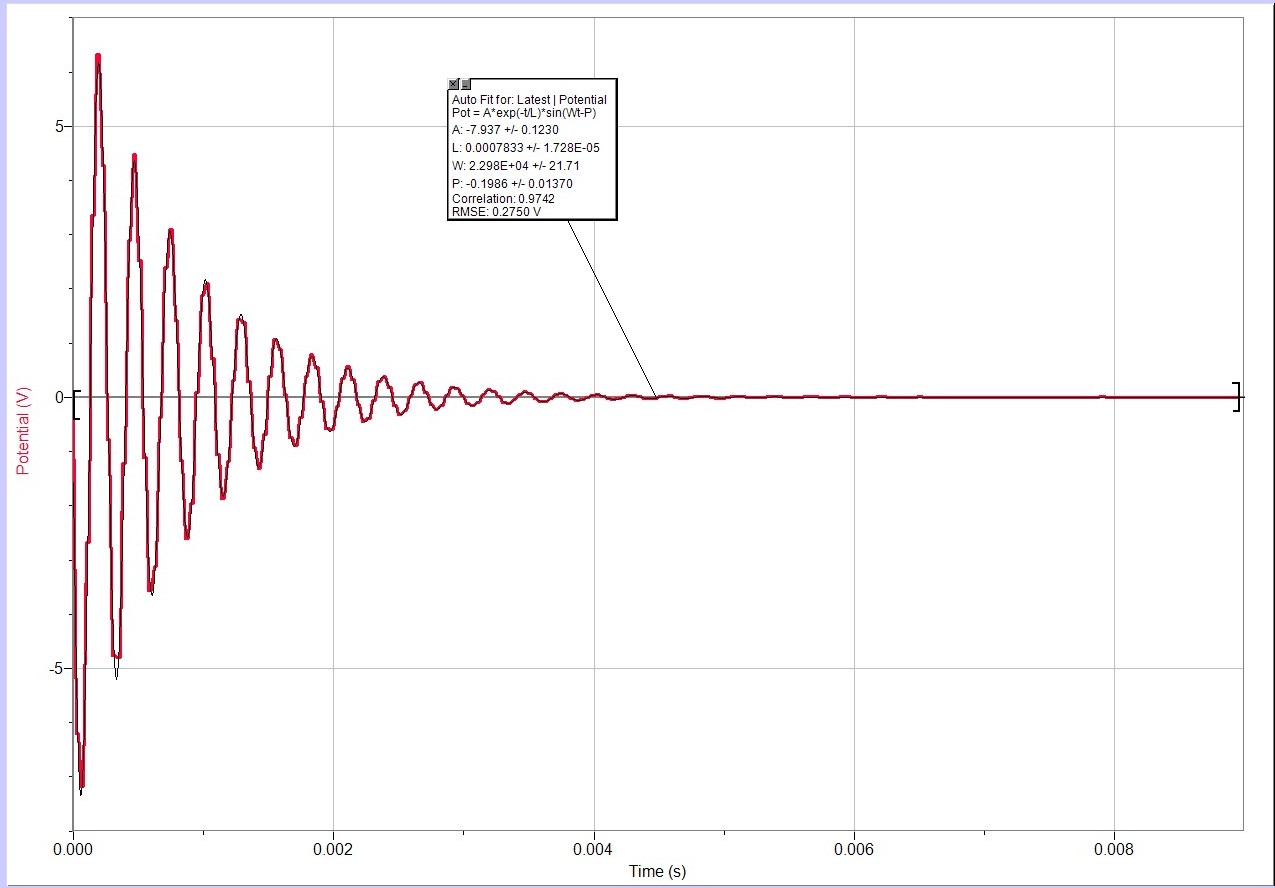
\includegraphics[width=0.7\textwidth]{figures/images/LCR_D1_Logger-Plot.jpg}
        \caption{Damped Oscillator plot using Logger Pro of the charge stored in a capacitor inside a circuit with a 0.022 $\mu$ F capacitor and no resistor. The capacitor was measured to have a capacitance of $0.022\pm0.001\mu$ F. There is also an $86.6\pm0.1$mH inductor in the circuit.}
        \label{fig:D1_022C_0R}
    \end{subfigure}
\end{figure}

\begin{figure} [h]
    \begin{subfigure}
        \centering
        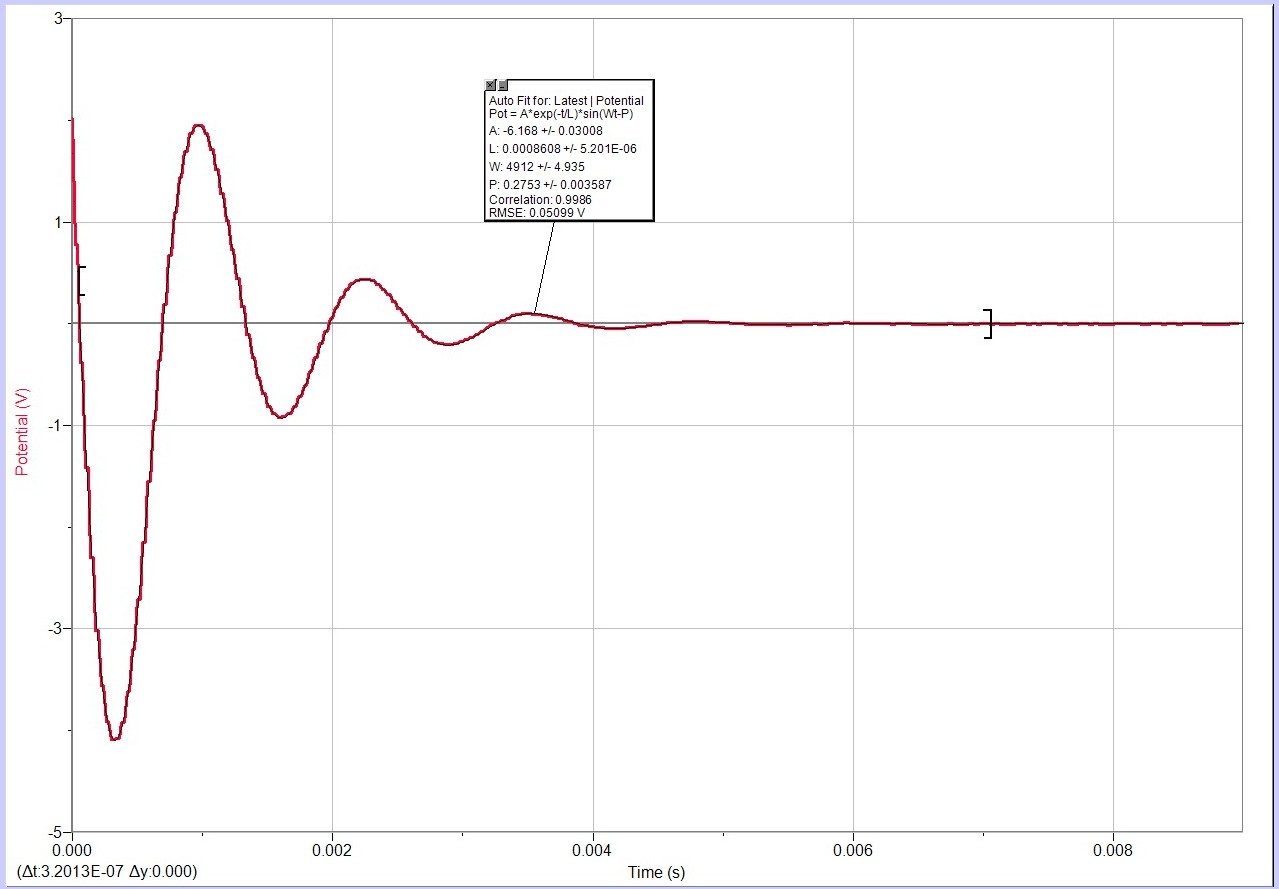
\includegraphics[width=0.7\textwidth]{figures/images/LCR_D2_Logger-Plot.jpg}
        \caption{Damped Oscillator plot using Logger Pro of the charge stored in a capacitor inside a circuit with a 0.47 $\mu$ F capacitor and no resistor. The capacitor was measured to have a capacitance of $0.47\pm0.01\mu$ F. There is also an $86.6\pm0.1$mH inductor in the circuit.}
        \label{fig:D2_47C_0R}
    \end{subfigure}
\end{figure}

\begin{figure} [h]
    \begin{subfigure}
        \centering
        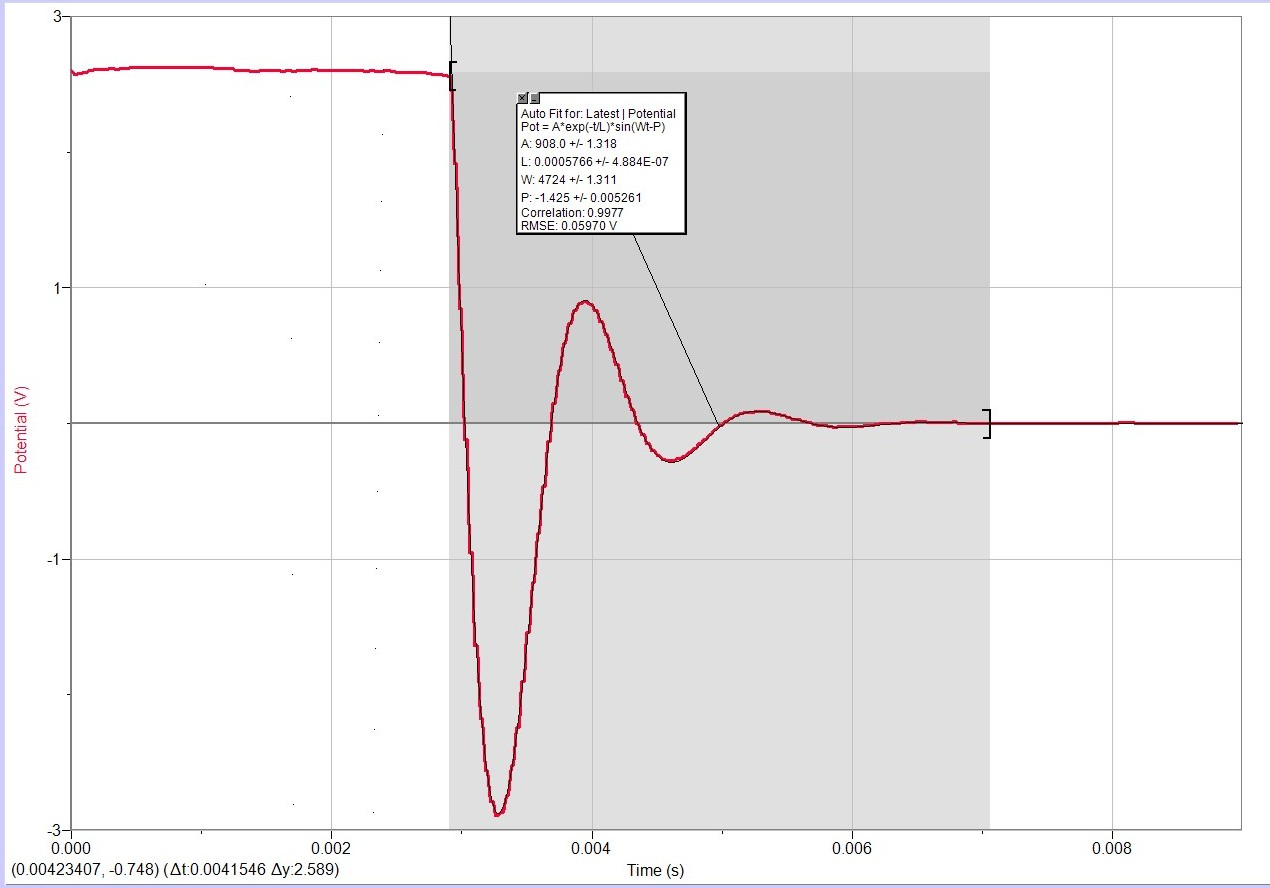
\includegraphics[width=0.7\textwidth]{figures/images/LCR_D3_Logger-Plot.jpg}
        \caption{Damped Oscillator plot using Logger Pro of the charge stored in a capacitor inside a circuit with a 0.47 $\mu$ F capacitor and a 100$\Omega$ resistor. The capacitor was measured to have a capacitance of $0.47\pm0.01\mu$ F, and the resistor was measured to have a resistance of $99.1\pm0.1\Omega$. There is also an $86.6\pm0.1$mH inductor in the circuit.}
        \label{fig:D3_47C_100R}
    \end{subfigure}
\end{figure}

\begin{figure} [h]
    \begin{subfigure}
        \centering
        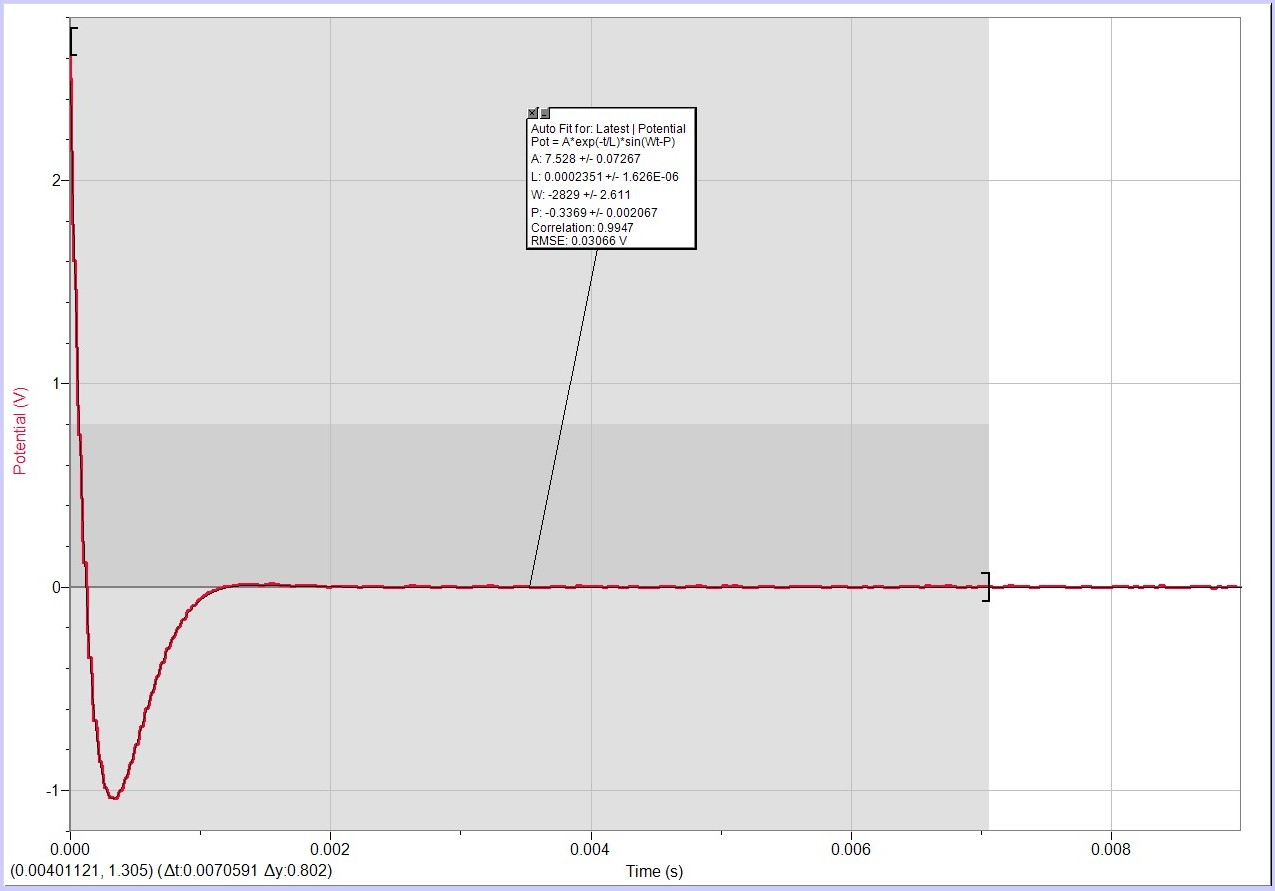
\includegraphics[width=0.7\textwidth]{figures/images/LCR_D4_Logger-Plot.jpg}
        \caption{Damped Oscillator plot using Logger Pro of the charge stored in a capacitor inside a circuit with a 0.47 $\mu$ F capacitor and a 500$\Omega$ resistor. The capacitor was measured to have a capacitance of $0.47\pm0.01\mu$ F, and the resistor was measured to have a resistance of $492.5\pm0.1\Omega$. This resistor was created by combining two resistors in parallel, measuring $0.99\pm0.01\text{k}\Omega$ and $0.98\pm0.01\text{k}\Omega$, respectively. There is also an $86.6\pm0.1$mH inductor in the circuit.}
        \label{fig:D4_47C_500R}
    \end{subfigure}
\end{figure}

\begin{figure} [h]
    \begin{subfigure}
        \centering
        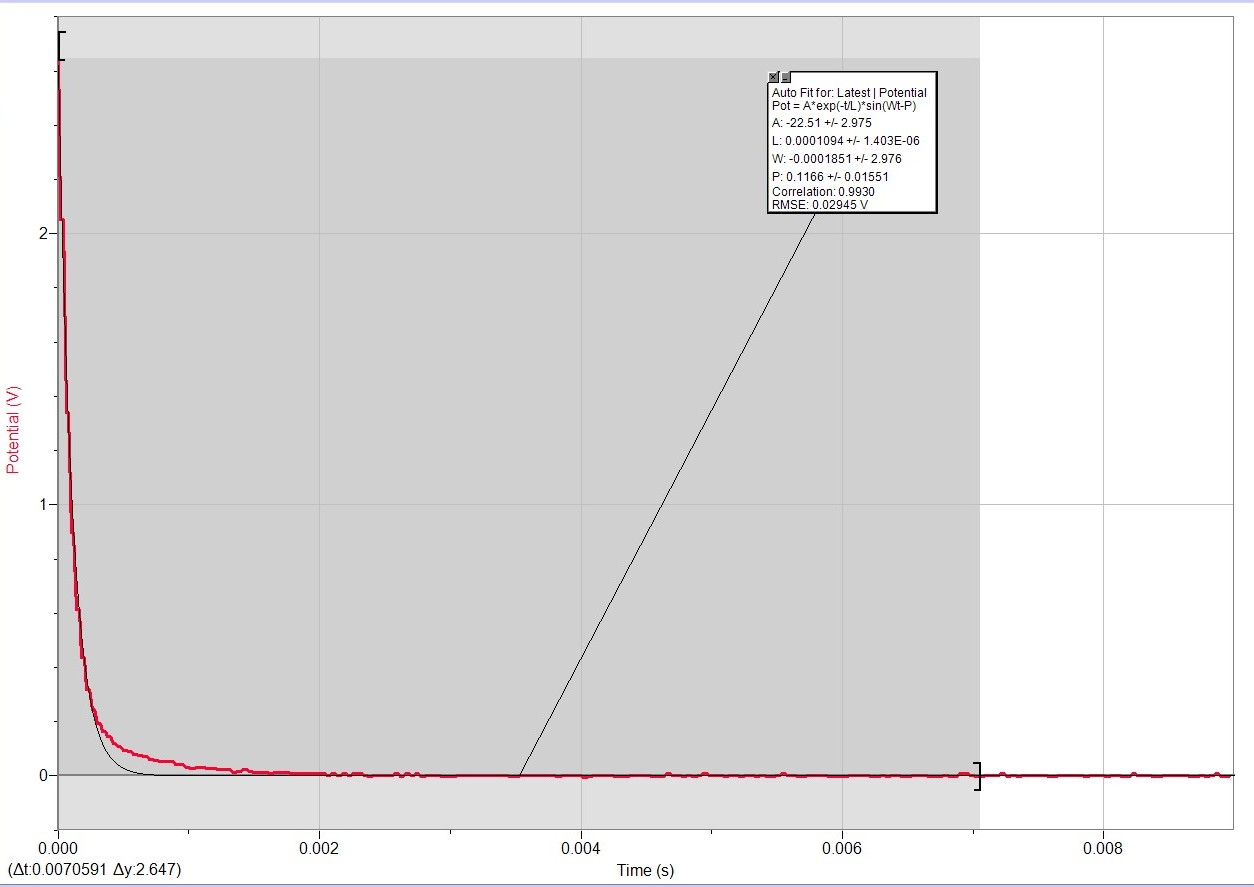
\includegraphics[width=0.7\textwidth]{figures/images/LCR_D5_Logger-Plot.jpg}
        \caption{Damped Oscillator plot using Logger Pro of the charge stored in a capacitor inside a circuit with a 0.47 $\mu$ F capacitor and a 1 k$\Omega$ resistor. The capacitor was measured to have a capacitance of $0.47\pm0.01\mu$ F, and the resistor was measured to have a resistance of $0.99\pm0.01\text{k}\Omega$. There is also an $86.6\pm0.1$mH inductor in the circuit.}
        \label{fig:D5_47C_1000R}
    \end{subfigure}
\end{figure}

\begin{figure} [h]
    \begin{subfigure}
        \centering
        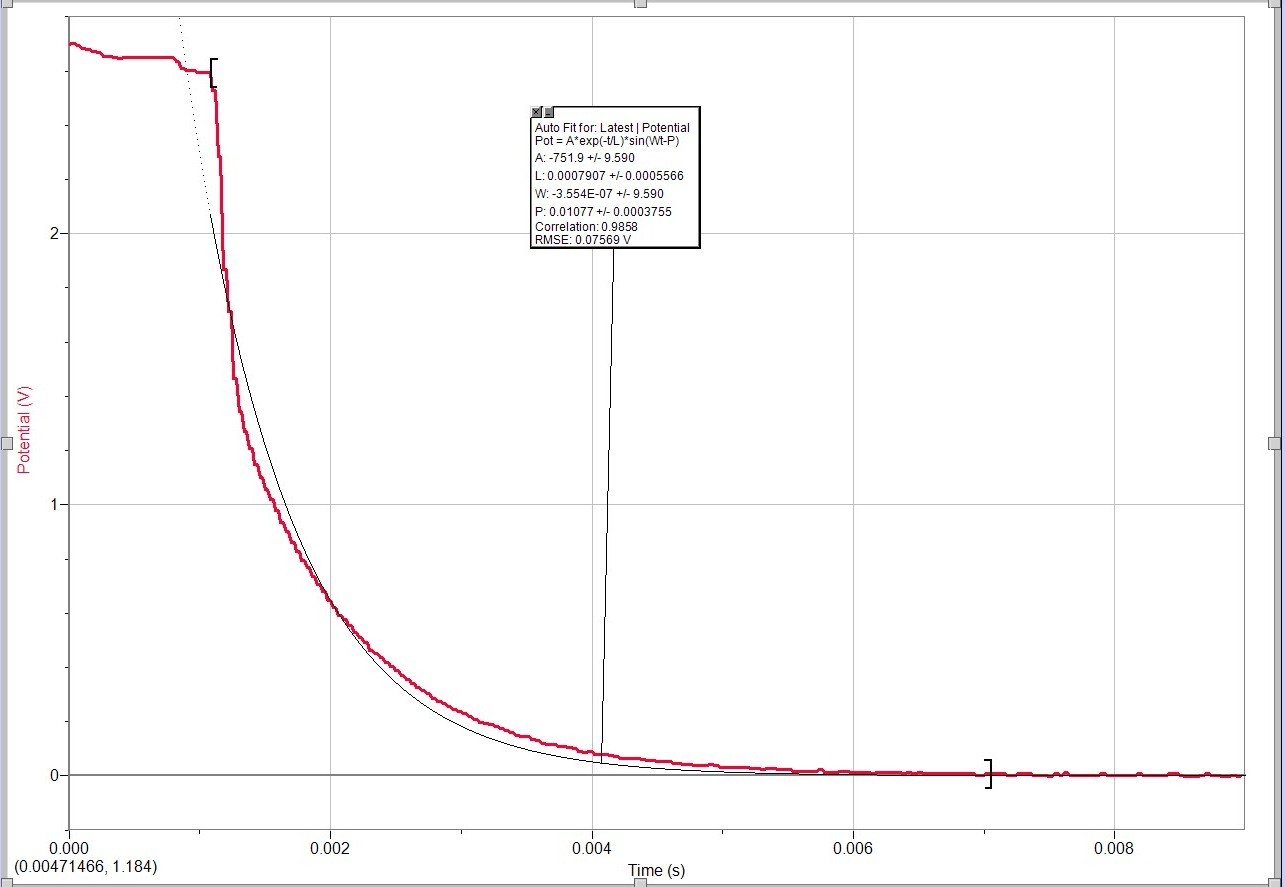
\includegraphics[width=0.7\textwidth]{figures/images/LCR_D6_Logger-Plot.jpg}
        \caption{Damped Oscillator plot using Logger Pro of the charge stored in a capacitor inside a circuit with a 0.47 $\mu$ F capacitor and a 1 k$\Omega$ resistor. The capacitor was measured to have a capacitance of $0.47\pm0.01\mu$ F, and the resistor was measured to have a resistance of $1.97\pm0.02\text{k}\Omega$. This resistor was created by combining two resistors in series, measuring $0.99\pm0.01\text{k}\Omega$ and $0.98\pm0.01\text{k}\Omega$, respectively. There is also an $86.6\pm0.1$mH inductor in the circuit.}
        \label{fig:D6_47C_2000R}
    \end{subfigure}
\end{figure}

\clearpage
\subsection{Resonant Circuit}

\begin{table}[h]
\centering
\begin{tabular}{|c|c|c|}
\hline
\textbf{Frequency (Hz)} & \textbf{Vpp (V)} & \textbf{Gain} \\
\hline
$2.25 \pm 0.01$  & $1.14 \pm 0.02$  & $0.07125 \pm 0.00125$ \\
$3.55 \pm 0.01$  & $2.02 \pm 0.02$  & $0.12625 \pm 0.00125$ \\
$4.85 \pm 0.01$  & $3.34 \pm 0.02$  & $0.20875 \pm 0.00125$ \\
$6.15 \pm 0.01$  & $5.10 \pm 0.02$  & $0.31875 \pm 0.00125$ \\
$7.45 \pm 0.01$  & $10.40 \pm 0.02$ & $0.65000 \pm 0.00125$ \\
$8.00 \pm 0.01$  & $10.96 \pm 0.02$ & $0.68500 \pm 0.00125$ \\
$8.75 \pm 0.01$  & $9.92 \pm 0.02$  & $0.62000 \pm 0.00125$ \\
$10.05 \pm 0.01$ & $6.88 \pm 0.02$  & $0.43000 \pm 0.00125$ \\
$11.35 \pm 0.01$ & $4.96 \pm 0.02$  & $0.31000 \pm 0.00125$ \\
$12.65 \pm 0.01$ & $3.92 \pm 0.02$  & $0.24500 \pm 0.00125$ \\
$13.95 \pm 0.01$ & $3.20 \pm 0.02$  & $0.20000 \pm 0.00125$ \\
$15.25 \pm 0.01$ & $2.72 \pm 0.02$  & $0.17000 \pm 0.00125$ \\
$16.55 \pm 0.01$ & $2.40 \pm 0.02$  & $0.15000 \pm 0.00125$ \\
$17.85 \pm 0.01$ & $2.16 \pm 0.02$  & $0.13500 \pm 0.00125$ \\
$19.15 \pm 0.01$ & $1.92 \pm 0.02$  & $0.12000 \pm 0.00125$ \\
$20.45 \pm 0.01$ & $1.76 \pm 0.02$  & $0.11000 \pm 0.00125$ \\
$21.75 \pm 0.01$ & $1.68 \pm 0.02$  & $0.10500 \pm 0.00125$ \\
$23.05 \pm 0.01$ & $1.52 \pm 0.02$  & $0.09500 \pm 0.00125$ \\
$24.35 \pm 0.01$ & $1.39 \pm 0.02$  & $0.08688 \pm 0.00125$ \\
$25.65 \pm 0.01$ & $1.31 \pm 0.02$  & $0.08188 \pm 0.00125$ \\
$26.95 \pm 0.01$ & $1.23 \pm 0.02$  & $0.07688 \pm 0.00125$ \\
$28.25 \pm 0.01$ & $1.18 \pm 0.02$  & $0.07375 \pm 0.00125$ \\
$29.00 \pm 0.01$ & $1.12 \pm 0.02$  & $0.07000 \pm 0.00125$ \\
\hline
\end{tabular}
\caption{Frequency vs. Vpp and Gain with uncertainties. Gain and its uncertainty is calculated by dividing the corresponding Vpp values by 16, the input voltage from the function generator. }
\label{tab:gain_freq}
\end{table}

\begin{figure} [h]
    \begin{subfigure}
        \centering
        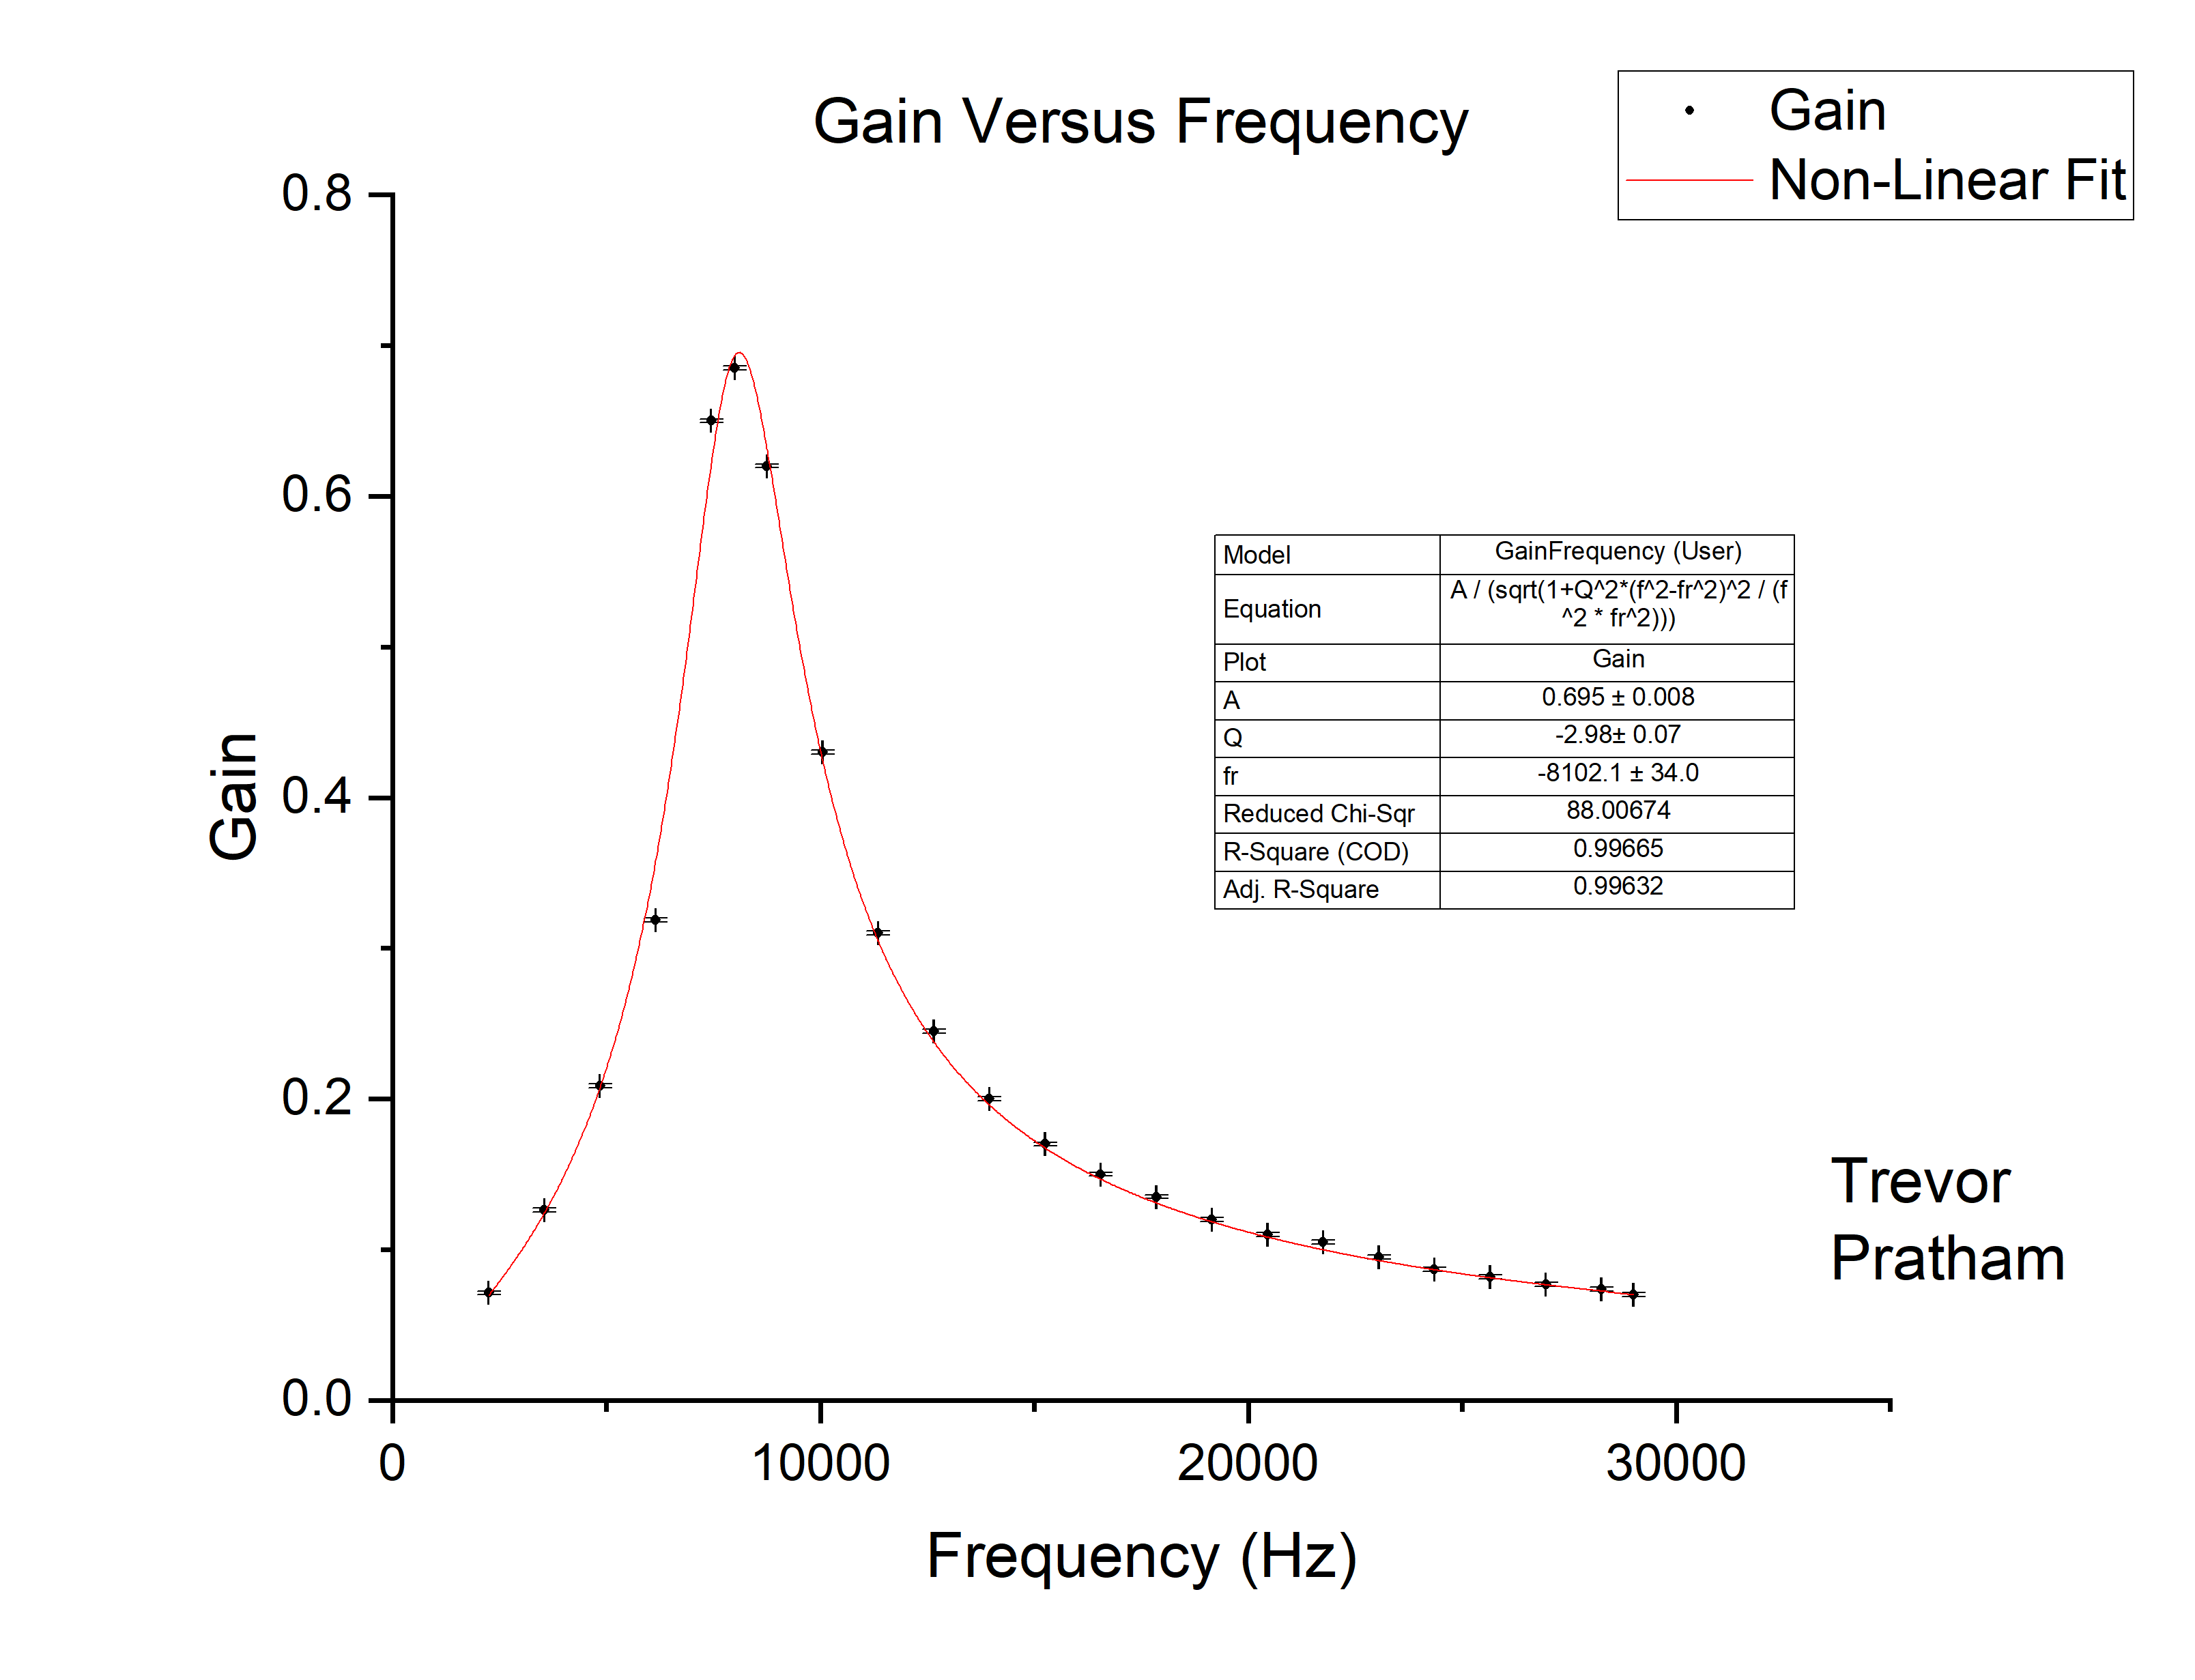
\includegraphics[width=0.7\textwidth]{figures/images/LCR_Gain-Frequency.png}
        \caption{Plot of Gain vs. Frequency from the above table (Table \ref{tab:gain_freq}). Non-linear fit was made using Origin, and the fitting equation along with its parameters are explained in the Theory section of this paper.}
        \label{fig:origin}
    \end{subfigure}
\end{figure}
\clearpage

\section{Other Calculations}
\subsection{Damped Oscillator}

\clearpage
\subsection{Resonant Circuit}

\end{document}
